\documentclass[a4paper]{llncs}
\usepackage[utf8]{inputenc}
\usepackage[english]{babel}
\usepackage{amssymb,amsfonts,amsmath}
\usepackage{graphicx}
\usepackage{alltt}
\usepackage{multicol}
%\usepackage[pdftex]{pstricks}
\usepackage{verbatim}
%\usepackage[font=small,labelfont=bf]{caption}
\usepackage{algorithmic}
\usepackage{algorithm}
\usepackage{xcolor}
\usepackage{synttree}
  \branchheight{0.3in}
  \childattachsep{1em}
  \childsidesep{1em}
%\usepackage[pdftex,colorlinks=true,plainpages=false]{hyperref}

%\usepackage[subtle,leading]{savetrees}
%\usepackage[subtle]{savetrees}
%\usepackage[moderate]{savetrees}

\newcommand{\url}[1]{{\tt #1}}

% Various useful commands for revisions...
\newcommand{\KILL}[1]{}
\newcommand{\HIDE}[1]{}

%\newtheorem{algorithm}{Algorithm}
\newcommand{\assign}{\leftarrow}
\renewcommand{\algorithmiccomment}[1]{~~// #1}

% abstract syntax
\newenvironment{datatype}{$\begin{array}{lcl}}{\end{array}$}
\newenvironment{grammar}{$\begin{array}{lcl}}{\end{array}$}
\newcommand{\is}{&\ ::=\ &}
\newcommand{\gen}{&\ \rightarrow\ &}
\newcommand{\alter}{\ \mid\ }
\newcommand{\altis}{\\ &\ \mid\ &}
%\newenvironment{action}{ & & \left\{\begin{array}{lcl}}{\end{array}\right.}
\newcommand{\laction}{\quad \{\ }
\newcommand{\baction}{\\ & & \left\{\begin{array}{lcl}}
\newcommand{\eaction}{\end{array}\right.}
\newcommand{\defby}{& := &}
\newcommand{\acode}[1]{\textrm{{\tt #1}}}
\newcommand{\concat}{~@@~}
\newcommand{\then}{\\ & @@ &}
\newcommand{\dtskip}{\end{array}$ $\begin{array}{lcl}}
\newcommand{\mathsc}[1]{\textrm{\sc #1}}

\newcommand{\nat}{\mathbb{N}}

\sloppy

%\pagestyle{plain}

\begin{document}

\title{An MDL-based Approach to the ARC Challenge}

\author{Sébastien Ferré}

\institute{Univ Rennes, CNRS, IRISA\\ %, Universit\'e de Rennes 1\\
  Campus de Beaulieu, 35042 Rennes, France\\
  Email: \email{ferre@irisa.fr}}

\maketitle

\begin{abstract}
\end{abstract}

%% keywords
\HIDE{
Measure of Intelligence
Artificial Intelligence
Explainable AI
Program Synthesis
Structured Prediction
Minimum Description Length
2D Parsing
}

\sloppy

\section{Introduction}
\label{intro}

This document describes our approach to the ARC (Abstraction and
Reasoning Corpus) challenge introduced by François Chollet as a tool
to measure intelligence, both human and artificial~\cite{Chollet2019}.
ARC was introduced in order to foster research on general artificial
intelligence, and to move from system-centric generalization to
developer-specific generalization. The latter enables a system to
``handle situations that neither the system nor the developer of the
system have encountered before''. For instance, a system trained to
recognize cats features system-centric generalization because it can
recognize cats that it has never seen, but in general, it does not
feature developer-aware generalization because it can not learn to
recognize horses with only a few examples (unlike a young child
would).

ARC is made of 1000 learning tasks, 400 for training, 400 for
evaluation, and 200 kept secret by its author in order to ensure
bias-free evaluation. Each task consists in learning how to generate
an output colored grid from an input colored grid (see
Figure~\ref{fig:task} of an example).
%
ARC is a challenging target for AI. As F. Chollet writes: ``to the
best of our knowledge, ARC does not appear to be approachable by any
existing machine learning technique (including Deep
Learning)''~\cite{Chollet2019}. The main difficulties are the
following:
\begin{itemize}
\item The expected output is not a label, or even a set of labels, but
  a colored grid with size up to 30x30, and with up to 10 different
  colors. It therefore falls in the domain of {\em structured
    prediction}~\cite{dietterich2008structured}.
\item The predicted output has to match exactly the expected
  output. If a single cell is wrong, the task is considered as
  failed. To compensate for that, three attempts are allowed for each
  input grids.
\item In each task, there are only between 2 and 4 training instances
  (input grid + output grid), and 1 or 2 test instances for which a
  prediction has to be made.
\item Each task relies on a distinct transformation from the input
  grid to the output grid. In particular, no evaluation task can be
  solved by reusing a transformation learned on the training
  tasks. Actually, each task is a distinct learning problem, and what
  ARC evaluates is broad generalization and few-shot learning.
\end{itemize}
A compensation for those difficulties is that the the input and output
data are much simpler than real-life data like photos or texts. We
think that this helps to focus on the core features of intelligence
rather than on scalability issues.

Our approach is based on the MDL (Minimum Description Length)
principle~\cite{Rissanen1978,Grunwald2019} according to which the best
model for some data is the one that compresses the most the data.
%
The MDL principle has already been applied successively to pattern
mining, classification, and clustering tasks~\cite{KRIMP2011}.
%
A major difference with those work is that the model to be learned
need not only explain the data but also be able to perform a
computation from an input data to an output data, here colored grids.

%%%
\section{Formalizing ARC Tasks}
\label{arc}

\begin{figure}[t]
  \centering
  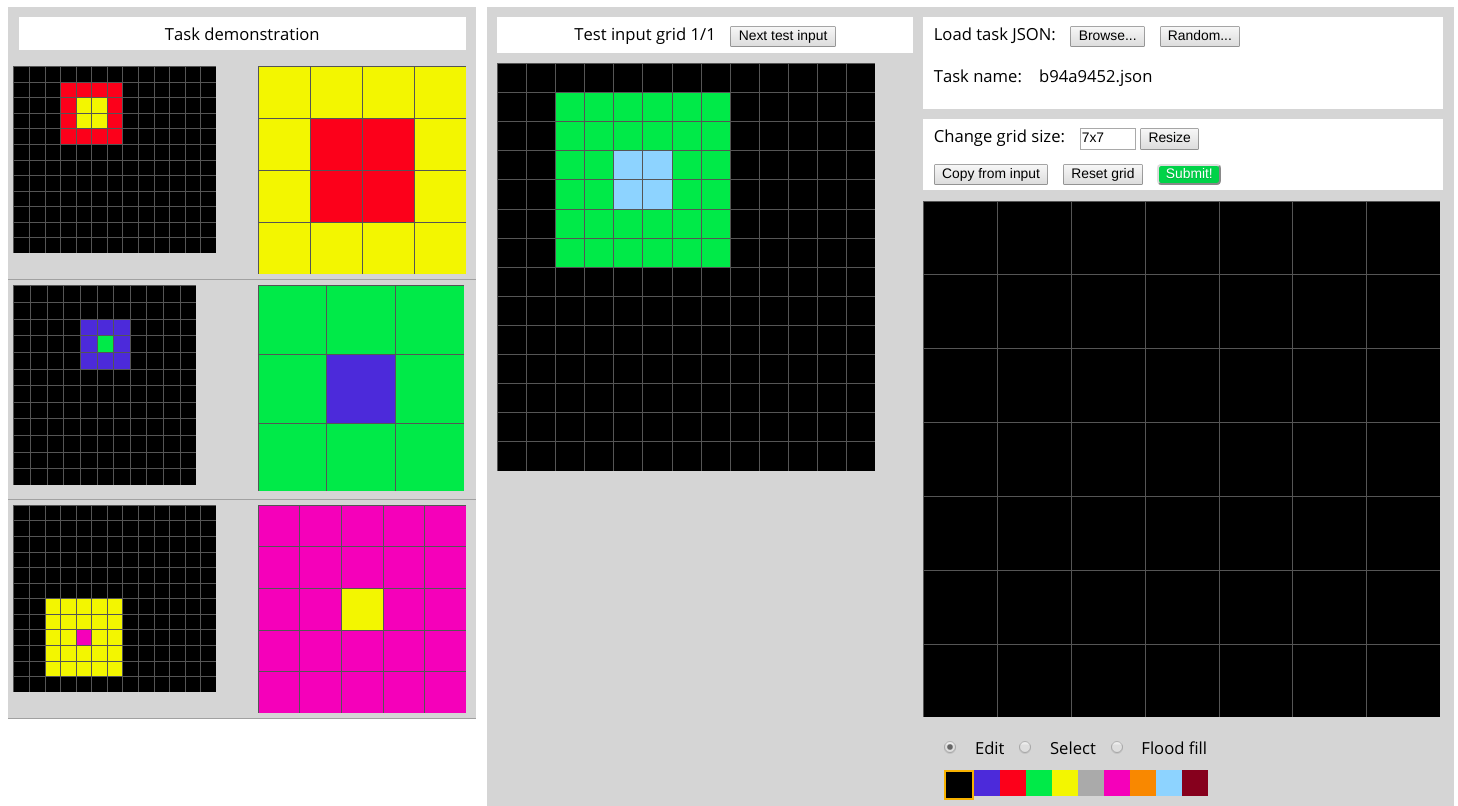
\includegraphics[width=\textwidth]{fig/training_b94a9452.png}
  \caption{One of the training tasks, with three examples on the left,
    a test input grid in the middle, and the widget that can be used
    to draw the corresponding output grid.}
  \label{fig:task}
\end{figure}

\begin{definition}[colors]
  We assume a finite set~$C$ of distinct symbols, which we call {\em colors}.
\end{definition}

In ARC, there are 10 colors coded by digits (0..9) in JSON files, and
by colors (e.g., black, purple, red) in the web interface (see
Figure~\ref{fig:task}).

\begin{definition}[grid]
  A {\em grid} $g \in C^{h \times w}$ is a matrix of colors with $h>0$
  rows, and $w>0$ columns. A grid is often displayed as a colored
  grid. The number of rows is called the {\em height} of the grid, and
  the number of columns is called the {\em width} of the grid.
  
  A {\em grid cell} is caracterized by {\em coordinates}~$(i,j)$,
  where $i$ selects a row, and $j$ selects a column. The color at
  coordinates~$(i,j)$ is denoted either by~$g_{ij}$ or by~$g[i,j]$.
  Coordinates range from~$(0,0)$ to~$(h-1,w-1)$.
\end{definition}

In ARC, grids have a size from (1,1) to (30,30).

\begin{definition}[example] 
  An {\em example} is a pair of grids~$e = (x,y)$, where $x$ is called
  the {\em input grid}, and $y$ is called the {\em output grid}.
\end{definition}

As illustrated by Figure~\ref{fig:task}, the output grid needs not
have the same size as the input grid, it can be smaller or bigger.

\begin{definition}[task]
  A {\em task} is a pair~$T = (E,F)$, where $E$ is the set of {\em
    training examples}, and $F$ is the set of {\em test examples}.
  The learner has access to the input and ouput grids of the training
  examples, but only to the input grids of the test examples. Its
  % TODO: wrong, no access to test input grids
  objective is to predict the hidden output grids of all test
  examples.
\end{definition}

As illustrated by Figure~\ref{fig:task}, the different input grids of
a task need not have the same size, nor use the same colors. The same
applies to test grids.

The ARC is composed of 1000 tasks in total: 400 for training, 400 for
evaluation by developers, and 200 for independent
evaluation. Figure~\ref{fig:task} shows one of the 400 training tasks,
with three training examples, and one test grid. Developers should
only look at the training tasks, not at the evaluation tasks, which
should only be used to evaluate the broad generalization capability of
the system.

Each task has between 2 and 4 training examples, and 1 or 2 test
examples.

%%%
\section{Modelling ARC Tasks as Two-Part MDL}
\label{modelling}

The objective is here to design a class of {\em task models} that can
be used to represent a transformation from input grids to output
grids.
%
Our key intuition is that a task model can be decomposed into two grid
models, one for the input grids, and another for the output grid. The
{\em input grid model} expresses what is common to all input grids,
while the {\em output grid model} expresses what is common to all
training output grids.
%
The actual transformation involves the two models as follows. The
input grid model is used to {\em parse} the test input grid, and the
parsing process produces some information that complements the input
model to fully specify that specific grid. Then, that parsing
information is fed into the output grid model in order to generate a
grid that matches the output model, and is also specific and related
to the input grid.

\subsection{Models}
\label{model}

The main component of grid models is {\em shapes}. Indeed, ARC grids
can often be read as various shapes over a background. Shapes can have
nested shapes, be adjacent or overlap with other shapes. Each shape
has a number of attributes (e.g., height, width, position, and color
for rectangles), which may be either constant over examples or
variable.

Given a shape, parsing a grid consists in finding its instances in the
grid, if any, and to return corresponding values for its variable
attributes. In contrast, generating a grid requires values for the
variable attributes as input in order to generate a shape instance in
the grid.

\paragraph{Version 1.} We define the first version of our model with
algebraic data types. 

\begin{center}
\begin{datatype}
  {\it task} \is {\bf InOut}({\it grid}, {\it grid})
  \\
  {\it grid} \is {\bf Background}(height: {\it attr}_\nat, width: {\it attr}_\nat, color: {\it attr}_C)
  \altis {\bf AddShape}({\it shape}, {\it grid})
  \\
  {\it shape} \is {\bf Rectangle}(height: {\it attr}_\nat, width: {\it attr}_\nat,\\
  & & \hspace*{1cm} mini: {\it attr}_\nat, minj: {\it attr}_\nat, color: {\it attr}_C)
  \\
  {\it attr}_\alpha \is {\bf Unkown}(ident)
  \altis {\bf Expr}({\it expr}_\alpha)
  \\
  {\it expr}_\alpha \is {\bf Var}(ident)
  \altis {\bf Const}(c: \alpha)
  \altis {\bf Plus}({\it expr}_\nat, {\it expr}_\nat), \alpha = \nat
  \altis {\bf Minus}({\it expr}_\nat, {\it expr}_\nat), \alpha = \nat
\end{datatype}
\end{center}

A task model is made of two grid models, one for the input grid,
another for the output grid.
%
Each grid model is a stack of shapes on top of a background. The
background is attributed with two integer attributes -- height and
width -- and a color attribute.
%
The only shape at this stage is the rectangle, attributed with four
integer attributes -- height, width, mini (with $i$ as a row index),
and minj (with $j$ as a column index) -- and a color attribute. The
height and width give the size of the rectangle, while mini and minj
give its position on the background.

An attribute is either an unknown -- with some identifier name -- or
an expression. The purpose of unknowns is to capture the variable
attributes of shapes during parsing. As a consequence, the output grid
model of a successful learned model should not contain
unknowns. However, as we show later, unknowns are also relevant in the
output grid models in the course of learning. We note $U(grid)$ the
set of unknowns in a grid model.
%
The purpose of expressions is to define attribute values as constant
over all examples, or as the result of a computation involving
variables. Parsing and generation of grids require that values are
given for those variables but each example may receive different
values for each variable. Complex expressions are typically used in
the output grid models, where variables match unknowns of the input
grid model, and their values come from the parsing of the input
grid. On the contrary, only constants are used in the input grid
models as they receive no other information than the input grid.  We
note $V(grid)$ the set of expression variables used in a grid model.

Index~$\alpha$ of ${\it attr}, {\it expr}$ is the type of attribute
and expression values. Hence the use of type~$\alpha$ in
${\bf Const}$, and the constraints $\alpha = \nat$ for constructors
${\bf Plus}, {\bf Minus}$.

A task model is {\em well-formed} if the input grid model has no
expression variable, and if all expression variables occuring in the
output grid model occur as unknowns in the input grid model. As
mentioned above, unknowns are allowed in the output grid model in
order to represent intermediate stages in the learning process. They
represent output attributes that are not yet explained in terms of
input attributes.

A task model is {\em effective} if it is well-formed, and the output
grid model has no unknown. Such a model can therefore be used to
generate output grids from the parsing of input grids. An effective
and correct model for the task in Figure~\ref{fig:task} is the
following (color~0 is black).
\[\begin{array}{l}
{\bf InOut}( \\
\quad {\bf AddShape}({\bf Rectangle}(?H_2,?W_2,?I_2,?J_2,?C_2), \\
\quad \quad {\bf AddShape}({\bf Rectangle}(?H_1,?W_1,?I_1,?J_1,?C_1), \\
\quad \quad \quad {\bf Background}(?H_0,?W_0,0))), \\
\quad {\bf AddShape}({\bf Rectangle}(H_2,W_2,I_2-I_1,J_2-J_1,C_1), \\
\quad \quad  {\bf Background}(H_1,W_1,C_2))) \\
\end{array}\]

\subsection{Data According to a Model}
\label{data}

A model captures regularities in data but is generally not enough to
capture all the information in data. In MDL-based approaches to model
selection it is essential to have a lossless encoding of data in order
to have a fair comparisons of different models.

Given a task and a task model, the question is: What minimum data
needs to be added to the task model in order to recover the task,
i.e. all input and output grids of the task.
%
Regarding input grids~$g^i_k$, for $k$ running through examples,
values must be given for each unknown in the input grid model~$m^i$,
and so for each task example~$k$. We call those {\em input
  parameters}~$\pi^i_k$. In the case where the input model and
parameters do not explain entirely the input grid, we also include as
data the list of cells that are different in the original grid and in
the model-generated grid. We call this the {\em input
  delta}~$\delta^i_k$. As a well-formed input grid model contains no
expression variable, there is no need to provide values for such
variables.

Regarding output grids~$g^o_k$, output parameters~$\pi^o_k$ and output
delta~$\delta^o_k$ must be provided similarly to input grids. In
well-formed models, no values for expression variables need to be
provided as they are provided by input parameters. The objective of
learning is to find a model with neither output parameters nor output
delta because in this case, the output grid is entirely determined by
the input grid.

More formally, a set of parameters is a partial mapping from
identifiers to values of various types (integers, colors). A delta is
a set of triples~$(i,j,c) \in \nat \times \nat \times C$ stating that
the cell at coordinates~$(i,j)$ has color~$c$ (instead of the color
specified by the grid model).

The data in Figure~\ref{fig:task} according to the above model has
empty input and output delta, as well as empty output parameters. The
input parameters are given in the following tables for the train input
grids.
\begin{center}
  \begin{tabular}{l|cccccccccccc}
    input grid & $H_0$ & $W_0$ & $H_1$ & $W_1$ & $I_1$ & $J_1$ & $C_1$ & $H_2$ & $W_2$ & $I_2$ & $J_2$ & $C_2$ \\
    \hline
    1 & 12 & 13 & 4 & 4 & 1 & 3 & 2 & 2 & 2 & 2 & 4 & 4 \\
    2 & 12 & 11 & 3 & 3 & 2 & 4 & 1 & 1 & 1 & 3 & 5 & 3 \\
    3 & 12 & 13 & 5 & 5 & 6 & 2 & 4 & 1 & 1 & 8 & 4 & 6 \\
    \hline
  \end{tabular}
\end{center}

\subsection{Parsing and Generating a Grid with a Grid Model}
\label{parsing}
\label{generating}

% schema of grid model
% involving: grid, env, model, params, delta 
% parsing: env, grid, model -> params, delta
% generating: env, model, params, delta -> grid

In MDL terms, {\em parsing} corresponds to the encoding of a grid into
parameters and delta with a grid model, while {\em generating}
corresponds the decoding of parameters and delta into a grid with a
grid model. To complete the picture, each process may also take as
input an additional set of parameters called {\em
  environment}~$\epsilon$, providing values for expression variables.
%
Formally, for every model~$m$, the parsing and generating processes
are functions with the following signatures:
\begin{itemize}
\item ${\it parse}_m : (\epsilon, g) \to (\pi, \delta)$,
\item ${\it generate}_m : (\epsilon, \pi, \delta) \to g$.
\end{itemize}

Parsing a grid works by first instantiating the model with the
environment, substituting expression variables by their value in the
environment, if defined. The resulting model is then matched over the
grid, thus providing values for the model unknowns,
i.e. parameters. Finally, cells that are not covered by the matching
are collected as the delta.  When several matchings are possible, the
one with the smallest delta should be chosen.

Generating a grid starts like parsing by instantiating the model with
the environment. Then, the model is further instantiated with
parameters, substituting the unknowns by their value in the
parameters. From there, a grid can be generated according to the
semantics of the model. Finally, the delta is applied to the grid,
possibly modifying some cells.

Parsing should be compatible with generating in the sense that
\[ \forall m, \epsilon, g: \exists \pi, \delta: {\it
    parse}_m(\epsilon,g) = (\pi,\delta) \Rightarrow {\it
    generate}_m(\epsilon,\pi,\delta) = g. \] The converse does not
necessarily hold in the sense that there may be several
pairs~$(\pi,\delta)$ generating the same grid~$g$. In practice, the
generating process is easier to implement than the parsing process
because while the former is rather straightforward, the latter can
have a high complexity.

\paragraph{Version 1.} In this first version, the parsing is
decomposed in three stages. First, the grid is partitioned into
contiguous monocolor regions. Second, rectangle shapes are looked for
as single parts or as unions of parts to cover the case where some
rectangle is overlaped by another shape. Third, matching
superpositions of rectangles are looked for according to the model.

For instance, the test input grid in Figure~\ref{fig:task} has three
contiguous parts: the light blue one, the green one, and the black
one. Three rectangles can be identified from those parts: a small
light blue square, a green rectangle overlaped by the blue one, and a
black rectangle covering the whole grid and overlaped by the other
rectangles. According to the above model, this input grid is parsed as
a 2x2 light blue rectangle at coordinates (3,4), on top of a 6x6 green
rectangle at coordinates (1,2), on top of a black background.

\subsection{Predicting Output from Input with a Task Model}
\label{predicting}

% TODO: schema showing the information flow
% involving: gi, mi, pi, di, mo, po, do

Using an effective task model~$m = (m^i,m^o)$ to predict the output
grid from the input grid simply consists into the composition of
parsing with the input grid model, and generating with the output grid
model.
\[ {\it predict}_m(g^i) := {\it
    generate}_{m^o}(\pi^i,\emptyset,\emptyset) \textrm{~s.t.~} \pi^i,
  \delta^i = {\it parse}_{m^i}(\emptyset, g^i) \] 
%
The input grid~$g^i$ is first parsed with the input grid model~$m^i$,
using an empty environment, which results in input parameters~$\pi^i$
and input delta~$\delta^i$. Then, the predicted grid is generated by
applying the output model~$m^o$ using the input parameters as
environment, and empty output parameters and delta. Output parameters
are not needed because the task model is effective.

For instance, given the parameters returned by the parsing of the test
input grid in Figure~\ref{fig:task}, the output grid model generates a
2x2 green rectangle at coordinates (2,2), on top of a 6x6 light blue
background, which is the expected grid.

%%%
\section{Learning Task Models}
\label{learning}

MDL-based learning works by selecting the model that compresses the
data the best. This involves two main components: (a) a measure of
compression so as to compare models, and (b) a strategy to explore the
model space. The measure of compression is called {\em description
  length}.

\subsection{Description Lengths}
\label{dl}

In two-part MDL, the description length (DL)~$L(M,D)$ measures the number
of bits required to communicate data~$D$ with model~$M$. It is
decomposed in two parts according to the equation
\[ L(M,D) = L(M) + L(D|M) \] where $L(M)$ is the DL of the model, and
$L(D|M)$ is the DL of the data encoded with the model.

In our case, $M$ is a task model~$m = (m^i,m^o)$, and the data is the
part~$T^-$ of a task~$T = (E,F)$ that is accessible to the learner
% TODO: we should have T- = E
(training examples and test inputs). We therefore have
\[ L(m,T^-) = L(m) + L(T^-|m). \]

The description length of the task model is the sum of the description
lengths of its two grid models.
\[ L(m) = L(m^i) + L(m^o) \] 
%
The description length of the task data boils down to the description
length of parameters and deltas:
\[\begin{array}{lcl}
L(T^-|m) & = & \alpha \sum_{e_k \in E} L_{m^i}(\pi^i_k) + L(\delta^i_k|h^i_k,w^i_k) + L_{m^o}(\pi^o_k) + L(\delta^o_k|h^o_k,w^o_k) \\
& + & \alpha \sum_{e_k \in F} L_{m^i}(\pi^i_k) + L(\delta^i_k|h^i_k,w^i_k), \\
  \end{array} \]
%
where for every example~$e_k = (x_k,y_k)$,
$x_k \in C^{h^i_k \times w^i_k}$, $y_k \in C^{h^o_k \times w^o_k}$,
$\pi^i_k, \delta^i_k = {\it parse}_{m^i}(\emptyset,x_k)$, and
$\pi^o_k, \delta^o_k = {\it parse}_{m^o}(\pi^i_k,y_k)$. For test
examples, the output terms are not included because output grids are
not accessible to the learner. We nonetheless include test input grids
in order to ensure that the learned model is applicable to them, and
% TODO: change that
also because it makes sense to use all of the available information.
%
Factor~$\alpha$ equals~1 by default but can be set to a higher value
to give more weights to the data, relative to the model, and hence
allow the learning of more complex models. Indeed, ARC tasks have a
very low number of examples (max. 4).

On output grids~$y_k$, we use parsing rather than generating. This is
explained by the fact that description lengths are used at the
learning stage rather than at the application stage. During learning,
output models are incomplete, and still require some parameters and
delta to generate the output grid~$y_k$. However, this output grid is
available during learning (for training examples), and using parsing
enables to find which parameters and delta are required. The objective
of learning is to make those output parameters and delta become
empty. Knowing what are the required parameters and delta can help the
learner improve the model in this direction.

Note that the description lengths of parameters are indexed by the
parametrized grid models. Indeed, knowing the grid model, we know the
number and types of parameters so that we can encode the parameter
values in a compact way, simply adding the description length of each
parameter value:
\[ L_m(\pi_k) = \sum_{(u,c) \in \pi_k} L_{m,u}(c). \] For every
model~$m$ and every unknown~$u$ in that model, $L_{m,u}$ is the
model-specific encoding for the unknown value. A model-independant
encoding should encode the number and types of parameters in addition
to the values. The model-specific encoding are defined along with the
escription length of models (see below).

The description length of deltas is parametrized by the height~$h$ and
width~$w$ of the encoded grid. This is valid because knowing the grid
model and the parameters, the size of the grid is known, and it only
remains to specify which of the grid cells need to be given a
different color. This leads to the following definition.
\[ L(h,w,\delta) = L_\nat(|\delta|) + log(C_{hw}^{|\delta|}) + |\delta|log(|C|-1) \]
%
The first term encodes the number of cells in the delta. The second
term encodes which cells in the grid ($hw$ cells in total) are in the
delta, using a combination. The third term encodes the colors of those
delta cells, choosing for each among the $|C|-1$ other colors, other
than the color generated with the model and parameters.

In the following we assume a few basic description lengths for
elementary types:
\begin{itemize}
\item $L_\nat(n) = 2\,log\ (n+1) + 1$: a universal encoding of natural
  intergers (including zero), more precisely the gamma encoding
  shifted by one to include zero;
\item $L_C = log\ |C|$: an encoding of colors along a uniform distribution.
\end{itemize}

%%% V1

\begin{table}[t]
\caption{Definition of the description length of models and their parameters}
\begin{center}
\begin{datatype}
  {\it task} \is {\bf InOut}({\it grid}_1, {\it grid}_2)
  \baction
  L(task) \defby L(grid_1,0) + L(grid_2,|U(grid_1)|)
  \eaction
  \\
  {\it grid} \is {\bf Background}(height: {\it attr}_\nat, width: {\it attr}_\nat, color: {\it expr}_C)
  \baction
  L(grid,N_V) \defby 1 + L(height,N_V,L_\nat) + L(width,N_V,L_\nat) + L(color,N_V,L_C)
  \eaction
  \altis {\bf AddShape}({\it shape}, {\it grid}_1)
  \baction
  L(grid,N_V) \defby 1 + L(shape,N_V) + L(grid_1,N_V)
  \eaction
  \\
  {\it shape} \is {\bf Rectangle}(height: {\it attr}_\nat, width: {\it attr}_\nat,\\
  & & \hspace*{1cm} mini: {\it attr}_\nat, minj: {\it attr}_\nat, color: {\it attr}_C)
  \baction
  L(shape,N_V) \defby L(height,N_V,L_\nat) + L(width,N_V,L_\nat) \\
  & + & L(mini,N_V,L_\nat) + L(minj,N_V,L_\nat) + L(color,N_V,L_C)
  \eaction
  \\
  {\it attr}_\alpha \is {\bf Unkown}(ident)
  \baction
  L(attr,N_V,L_\alpha) \defby 1 \\
  L_{m,ident}(c) \defby L_\alpha(c)
  \eaction
  \altis {\bf Expr}({\it expr}_\alpha)
  \baction
  L(attr,N_V,L_\alpha) \defby 1 + L(expr,N_V,L_\alpha)
  \eaction
  \\
  {\it expr}_\alpha \is {\bf Var}(ident)
  \baction
  L(expr,N_V,L_\alpha) \defby -log\ 0.3 + log\ N_V
  \eaction
  \altis {\bf Const}(c: \alpha)
  \baction
  L(expr,N_V,L_\alpha) \defby -log\ 0.5 + L_\alpha(c)
  \eaction
  \altis {\bf Plus}({\it expr}_1, {\it expr}_1)
  \baction
  L(expr,N_V,L_\alpha) \defby -log\ 0.1 + L(expr_1,N_V,L_\alpha) + L(expr_2,N_V,L_\alpha)
  \eaction
  \altis {\bf Minus}({\it expr}_1, {\it expr}_2)
  \baction
  L(expr,N_V,L_\alpha) \defby -log\ 0.1 + L(expr_1,N_V,L_\alpha) + L(expr_2,N_V,L_\alpha)
  \eaction
\end{datatype}
\end{center}
\label{tab:l:v1}
\end{table}

\paragraph{Version 1.} Table~\ref{tab:l:v1} defines the description
length (DL) of models (version~1), and of their
parameters. Function~$L$ is defined for all types, and for each type
variants. Depending on each type, it may take additional
parameters. The DL of a model is essentially the sum of the DLs of its
components. When there are several variants in a type, bits are added
to encode which variant applies. For types $grid$ and $attr$, 1 bit is
used as there are two variants; for type~$expr$, the number of bits is
derived from a probability distribution, giving more weight to
constants and variables than to addition and substraction.

The DL of a grid model depends on the number~$N_V$ of variables in its
environment, 0 for the input grid model, and the number of input
unknowns for the output grid model. This number~$N_V$ is passed down
to expression variables, which use it to encode a variable according to a
uniform distribution among the $N_V$ environment variables.

The DL of attributes and expressions, as they are generic in the type
of values, take as parameter a function~$L_\alpha$ for the encoding of
constants of that type (typically $L_\nat$ for integers, and $L_C$ for
colors).

Unknowns are encoded with a single bit in the model, to encode the
choice between an unknown and an expression. The encoding of their
values is delayed to the encoding of the grid model parameters~$\pi$,
as part of ``data according to the model''.  Function~$L_{m,ident}$
defines the DL of that delayed encoding for the unknown named
$ident$. It is here simply defined as the constant DL~$L_\alpha$ but
refinements are possible based on the knowledge of the grid model as
prior. For instance, uniform encoding can be used instead of universal
encoding for integers when bounds are known for the attribute value
(e.g., grid size).

For the task in Figure~\ref{fig:task}, the following table compares
the description lengths of the initial model and the above example
model, for $\alpha=10$ (each example counts as 10). The split between
the model and data according to the model is also given.

\begin{center}
  \begin{tabular}{|l|r|r|r|}
    \hline
    model & $L(m)$ & $L(T^-|m)$ & $L(m,T^-)$ \\
    \hline
    initial & 8.0 & 5394.4 & 5402.4 \\
    example & 96.0 & 1487.6 & 1583.6 \\
    \hline
  \end{tabular}
\end{center}

The increase in the model DL is largely compensated by the data DL.


\subsection{Learning Strategy}

The model space is generally too vast for a systematic exploration,
and heuristics have therefore to be employed to guide the search for a
good model.
%
The learning strategy consists in the iterative refinement of models,
starting with an initial model, in search for the best model, i.e. the
most compressive model. Given a class of models, a search strategy is
therefore entirely specified by:
\begin{enumerate}
\item an initial model~$m_o$ ({\em initial model}), generally the
  simplest one;
\item and a function~$R$ mapping each model~$m$ to an ordered
  list~$m_1, m_2, \ldots$ of refined models ({\em refinements}),
  generally taking into account the data according to the model (here,
  grids, parameters and delta).
\end{enumerate}
We call a refinement~$m_i$ {\em compressive} if it reduces the
description length of the original model~$m$. The ordering of
refinements is important because the number of possible refinements
could be huge, and it has a cost to evaluate each refinement by
measuring its description length. Indeed, this involves the parsing of
both input and output grids by each refined model.  This ordering is
therefore a key part of the heuristics.

Another part of the heuristics consists in bounding the number of
compressive refinements per model that are considered, and the number
of models that are kept after each iteration. A {\em greedy search}
selects the first compressive refinement, and has therefore a single
model at each iteration. A {\em beam search} provides a wider
exploration by selecting $K_r$ compressive refinements per model, and
then selecting among them the $K_m$ best models for the next
iteration. $K_m$ is the beam width. The search halts when no
compressive refinement can be found.
% TODO: think again about strategy, look at beam stack search for instance, anytime+backtracking... complete if enough time

\paragraph{Version 1.} The initial model is made of two minimal grid
models, reduced to a background with unknown size and color.
\[ {\bf InOut}({\it Background}(H_1,W_1,C_1), {\it
    Background}(H_2,W_2,C_2)) \] Capital letters represent unknowns.

Two kinds of refinements are used: (1) addition
of a shape to a grid model (input or output), and (2) replacing
unknowns by an expressions in a grid model. As the only shape in this
version is the rectangle, the first kind of refinement consists in
inserting a new rectangle on top of the stack of rectangles, or at
some depth up to 3. The inserted rectangle is completely unspecified
in the sense that new unknowns are created for all of its attributes
(size, position, and color).

The second kind of refinement enables to specify those unknowns by
replacing them with expressions, i.e. either constants or computations
involving constants and environment variables. For the input grid
model, it can only be constants because the environment is empty. For
the output grid model, input unknowns are available as environment
variables. We only consider complex expressions for integers, and with
a form among $x$, $x+c$, $x-c$, $x+y$, $x-y$, for environment
variables~$x,y$, and a constant~$c$. We use input and output
parameters in order to identify which (unknown,expression) pairs are
so that both have the same value over all example grids. When an input
unknown is replaced by a constant, its occurences in the output grid
model (if any) as expression variables also have to be replaced by
that constant.

A tentative ordering of refinements is the following: input
expressions, input shapes, output expressions, output shapes. Among
expressions, the ordering is: $c$, $x$, $x+c$, $x-c$, $x+y$, $x-y$.

The sequence of compressive refinements that leads to the above model
about task in Figure~\ref{fig:task} is shown in the table below,
giving after each refinement the new values for description
lengths. For concision, successive unknown replacements are aggregated
into a single step.

\begin{center}
  \begin{tabular}{|c|l|r|r|r|}
    \hline
    step & refinement & $L(m)$ & $L(T^-|m)$ & $L(m,T^-)$ \\
    \hline
    0 & ${\bf InOut}({\it Background}(H_1,W_1,C_1),$ & & & \\
    & \hspace*{1.1cm}${\it Background}(H_2,W_2,C_2))$ & 8 & 5394 & 5402 \\
    1 & $C_1 \leftarrow 0$ & 9 & 5390 & 5399 \\
    2 & ${\bf Rectangle}(H_3,W_3,I_1,J_1,C_3)$ on top of $m^i$ & 16 & 2651 & 2667 \\
    3 & ${\bf Rectangle}(H_4,W_4,I_2,J_2,C_4)$ on top of $m^i$ & 25 & 2476 & 2501 \\
    4 & $H_2 \leftarrow H_3, W_2 \leftarrow W_3, C_2 \leftarrow C_4$ & 43 & 1951 & 1994 \\
    5 & ${\bf Rectangle}(H_5,W_5,I_3,J_3, C_5)$ on top of $m^o$ & 50 & 1819 & 1869 \\
    6 & $H_5 \leftarrow H_4, W_5 \leftarrow W_4,, C_5 \leftarrow C_3$ & & & \\
     & \hspace*{1cm} $I_3 \leftarrow I_2-I_1, J_3 \leftarrow J_2-J_1$ & 96 & 1488 & 1584 \\
    \hline
  \end{tabular}
\end{center}


%%%
\section{Evaluation}
\label{eval}

\KILL{
\begin{table}[t]
  \centering
  \caption{Performance on training and evaluation tasks, per version}
  \begin{tabular}{|c|c|c|c|c|c|}
    \hline
     & & \multicolumn{3}{|c|}{training} & evaluation \\
    ~Version~ & ~timeout~ & ~no output~ & ~wrong output~ & ~correct~ & ~correct~ \\
    \hline
    v1 & 1s & 278 & 116.5 & 5.5 & 0 \\
    \hline
  \end{tabular}
  \label{tab:eval}
\end{table}

For evaluation tasks, we only report the number of correct
predictions (among the 400 tasks) in order to avoid leaking
information from the evaluation dataset to the developer. For training
tasks, we provide finer results by splitting the 400 tasks in three
categories:
\begin{itemize}
\item {\bf no output}: no effective model could be found in the
  timeout;
\item {\bf wrong output}: an effective model could be found but there
  is a discrepancy between the predicted output and the expected
  output;
\item {\bf correct}: an effective model could be found, and predicts
  the expected output.
\end{itemize}
In results, half tasks appear because some tasks have two test
instances. If one test is correct, and another is wrong, we count 0.5
for each test. This enables to give the same weight to each task.
}%KILL

\begin{table}[t]
  \centering
  \caption{Performance on training and evaluation tasks as the number of tasks solved, per version}
  \begin{tabular}{|c|c|c|c|c|c|c|c|c|}
    \hline
     & & & & \multicolumn{2}{c|}{training} & \multicolumn{2}{c|}{evaluation} \\
    version & $\alpha$ & timeout & avg. time & train & test & train & test \\
    \hline
    v1 & ~10~ & 20s & 9s & ~9 / 9.6~ & ~5 / 5.5~ & ~0 / 0.3~ & ~0 / 0.0~ \\
    \hline
  \end{tabular}
  \label{tab:eval}
\end{table}

Table~\ref{tab:eval} reports on the performance of our approach on
both training and evaluation tasks (400 tasks each). A timeout is set
for each task. On both collections of tasks, we provide performance
for train examples, for which output grids are known, and for test
examples. In each case, we give two measures $n_1/n_2$: $n_1$ is the
number of tasks for which {\em all} examples are correctly solved, and
$n_2$ is the sum of partial scores over tasks. For instance, if a task
has two test examples and only one is solved, the score is~$0.5$.

\paragraph{Version 1.} This first version was designed by looking at
tasks {\tt ba97ae07} and {\tt b94a9452}. Evaluating it on training
tasks has shown that this simple model manages to solve 3.5 additional
tasks: {\tt 6f8cd79b}, {\tt 25ff71a9} (2 correct cases), {\tt
  5582e5ca}, {\tt bda2d7a6} (1 correct cases out of 2). This version
even manages to explain all train examples of 3 additional tasks,
hence 8 tasks in total, although they fail on the related test
examples: tasks {\tt a79310a0} (3 examples), {\tt bb43febb} (2
examples), {\tt 694f12f3} (2 examples), and {\tt a61f2674} (2
examples). For task {\tt a79310a0}, v1 recognizes that a shape is
moved, and changes color but, whereas all train shapes are rectangles,
the test shape is not a rectangle. For tasks {\tt bb43febb} and {\tt
  694f12f3}, v1 finds unplausible expressions to replace some
unknowns, e.g. replacing some height by a position instead of a height
decremented by a constant, or replacing some unknown by a constant
that happens to be valid for train examples but not for the test
example. For task {\tt a61f2674}, v1 is not powerful enough but given
that there are only two train examples, it manages to find some ad-hoc
regularity.

Despite those encouraging result on training tasks, no evaluation task
could be solved with this version. We wonder whether this is a
statistical fluke or the fact that evaluation tasks are harder than
the training tasks.

%%%
\section{Conclusion and Perspectives}
\label{conclu}

\bibliographystyle{splncs}
\bibliography{/local/ferre/recherche/biblio/bib}

\end{document}
